\chapter{Conceptual Framework for GenAI-Driven Security Automation}
\label{chap:conceptual_framework}

This chapter introduces the conceptual framework designed to address the critical challenges of automated security analysis and policy generation for cloud infrastructure. The proposed architecture presents a comprehensive, multi-layered approach that systematically processes \gls{iac} artifacts and automatically generates corresponding security policies. At its core, the framework leverages the power of traditional static analysis tools and advanced \glspl{llm} to create a robust security automation pipeline.

\section{Architectural Overview of the Proposed Framework}
\label{sec:architectural-overview}

The proposed architecture is founded on a hybrid model intentionally designed for efficacy, combining the reliability of established security scanners for identifying known vulnerability patterns with the contextual intelligence of generative AI \cite{khanna_enhancing_2024}. This approach allows for deeper analytical capabilities, necessary for uncovering complex, context-dependent security issues that traditional tools often miss \cite{akiri_generative_2025}. Furthermore, the architecture is conceived for seamless integration into modern \gls{devops} workflows, particularly \gls{cicd} pipelines, to operationalize a \gls{pac} model and enforce security throughout the development lifecycle \cite{khanna_enhancing_2024}.

As illustrated in Figure~\ref{fig:prototype-architecture}, the framework operates as a cohesive GenAI Security System triggered by external development workflows. The process begins when a \gls{cicd} pipeline initiates the workflow, providing \gls{iac} artifacts to the Ingestion Layer. This layer consumes the raw configurations and prepares them for analysis. The data is then passed to the Analysis Layer, which performs a two-stage evaluation. First, a Static Analysis component generates a baseline vulnerability report. This report is then fed into the GenAI Analysis component, which queries a curated Knowledge Base to produce an enriched, context-aware report, reducing false positives and identifying nuanced flaws.

\begin{figure}[htbp]
    \centering
    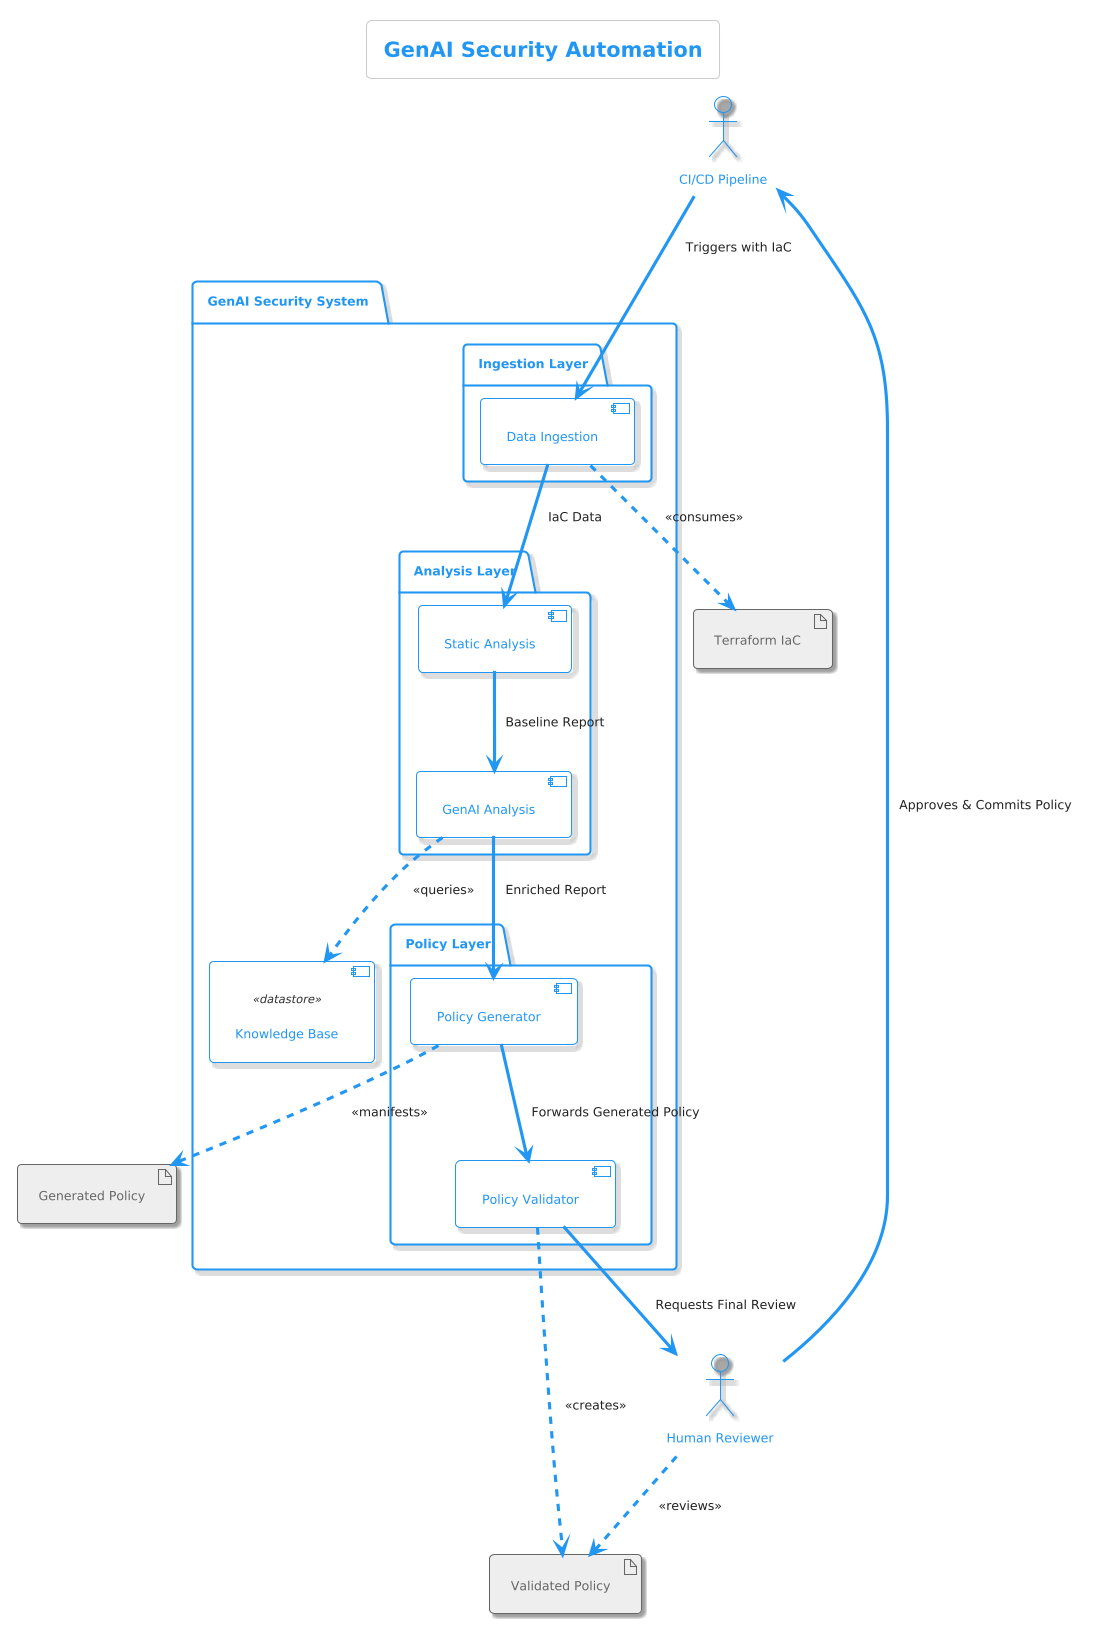
\includegraphics[width=0.95\textwidth]{Figures/component-abstract.png}
    \caption{Component Diagram of the Proposed GenAI-Driven Security Automation Framework}
    \label{fig:prototype-architecture}
\end{figure}

The enriched findings proceed to the Policy Layer, where the Policy Generator component leverages both the enriched report and the Knowledge Base to manifest a preventative Generated Policy. This artifact is immediately forwarded to a Policy Validator for automated checks. Following validation, the policy is presented to a Human Reviewer, a critical step that ensures oversight. Once approved, the now Validated Policy is committed back to the repository by the \gls{cicd} pipeline, closing the loop. This layered design provides a comprehensive and efficient system for enhancing cloud security posture by translating identified vulnerabilities directly into enforceable controls \cite{fakih_llm4cve_2025}. The following subsections will detail the specific roles and functions of each of these core layers.

\subsection{Ingestion Layer} % (fold)
\label{subsec:data-ingestion-layer}

The Data Ingestion Layer serves as the foundational entry point for security artifacts into the automation framework. Its primary function is to ingest \gls{iac} configurations, a prevalent standard for provisioning and managing cloud infrastructure. The reliance on \gls{iac}, while enhancing automation and consistency, introduces significant risks such as misconfigurations, coding errors, and embedded secrets, making automated analysis a critical requirement for secure cloud operations.

This layer is designed to support both batch and real-time ingestion modes, a flexible approach that aligns with modern data pipeline architectures emphasizing scalability and performance\cite{alevizos_towards_2024}. Batch ingestion allows for comprehensive, scheduled scans of entire code repositories, while real-time ingestion facilitates immediate analysis within \gls{cicd} pipelines \cite{gunathilaka_context-aware_2025}. The framework is designed to receive these \gls{iac} configurations via programmatic interfaces, ensuring seamless integration into existing developer workflows and automated systems.

Upon ingestion, the Data Ingestion Layer reads and parses the raw \gls{iac} configuration files, transforming them into a structured format suitable for further analysis. This foundational step ensures that the input artifacts are normalized and ready for systematic evaluation. Once parsing is complete, the processed configurations are handed off to the subsequent Analysis Layer, where both static and GenAI-driven analyses are performed to identify vulnerabilities and misconfigurations. The following subsection details the design and operation of this core analytical component.

\subsection{Analysis Layer}
\label{subsec:analysis-layer}

Following the Data Ingestion Layer, the Analysis Layer is responsible for the core analysis of the ingested \gls{iac} artifacts. A central design principle of this framework is the segregation of processing activities into two distinct but complementary sub-layers: a traditional Static Analysis Engine and an advanced \gls{genai} Analysis Engine.

The rationale for this dual-layer architecture is to create a highly efficient and comprehensive security analysis pipeline. This approach leverages the respective strengths of each technology. Static analysis provides a rapid, reliable, and computationally inexpensive method for identifying a wide range of known, pattern-based vulnerabilities. By filtering out these common issues first, the framework can then employ the more resource-intensive \gls{genai} engine to focus on complex, context-dependent security flaws that traditional tools are ill-equipped to detect \cite{zhang_empirical_2024}. This layered methodology optimizes analytical depth while maintaining operational efficiency, ensuring that both well-defined and nuanced vulnerabilities are addressed \cite{khanna_enhancing_2024}.

The first stage of this layer employs a suite of established \gls{sast} tools to conduct an initial scan of the \gls{iac} configuration. This engine examines the configuration for syntactic and structural flaws by referencing curated databases of known vulnerabilities, common misconfigurations, and code smells. It validates the configuration against established security benchmarks and standards. The primary output of this stage is a baseline vulnerability report, which provides a structured list of potential issues identified through deterministic, rule-based pattern matching. This report serves as a foundational input for the subsequent, more sophisticated analysis stage.

The second stage is the \gls{genai} Analysis Engine, which represents the core innovation of this framework and directly addresses the research interest in applying generative \gls{ai} to cloud security. This engine utilizes \glspl{llm} to perform a deeper, contextual analysis that transcends the limitations of traditional static scanners \cite{noauthor_artificial_2025}. It takes as input both the original \gls{iac} configuration and the baseline vulnerability report from the previous stage, using the initial findings to enrich its analytical context \cite{noauthor_towards_2025}.

This engine is designed to identify security weaknesses that require an understanding of developer intent, architectural relationships, and complex business logic \cite{noseevich_towards_2015}. Its capabilities include:

\begin{itemize}
\item \textbf{Identifying Context-Sensitive Flaws:} Detecting risks that emerge from the interaction of multiple configurations. For example, overly permissive network rules may appear acceptable in isolation but create a vulnerability when combined with a specific resource's placement within the network architecture\cite{zhang_empirical_2024}.
\item \textbf{Uncovering Logical and Policy Violations:} Identifying logical flaws in resource deployments, such as potential circular dependencies. The engine can also detect violations of complex, unwritten organizational policies like nuanced tagging and naming conventions \cite{khanna_enhancing_2024}.
\item \textbf{Reducing False Positives:} Differentiating between genuine security risks and findings from the static analysis that are benign within a specific operational context. For example, a "hardcoded secret" may simply be a placeholder for a non-production environment.
\end{itemize}

By synthesizing information from the configuration and the initial scan, the \gls{genai} Analysis Engine bridges the gap between traditional, rule-based detection and adaptive, context-aware threat identification, producing a consolidated and enriched vulnerability report.

\subsection{Policy Layer}
\label{subsec:policy-layer}

The Policy and Validation Layer operationalizes the insights derived from the Analysis Layer, acting as the primary action-oriented component of the framework. Its purpose is to automate the creation of security artifacts in the context of this prototype, preventative policies using \gls{genai}. This layer directly addresses a core aspect of this research: leveraging \glspl{llm} to not only analyze but also actively generate security policies. The integration of \gls{genai} into the security architecture in this manner marks a significant shift, promising to streamline development workflows and accelerate remediation cycles.

This layer leverages \glspl{llm} to generate security policies tailored to the vulnerabilities identified in the preceding analysis stages. The generated artifacts are formal policies written in a declarative, machine-readable language, designed for automated enforcement. The \gls{llm} is guided by system prompts and a curated knowledge base of security standards to produce precise, context-aware rules. This process of generating platform-specific policies from a higher-level analysis aligns with established methods in automated systems engineering, where abstract requirements are translated into concrete, executable artifacts for a target platform\cite{fakih_llm4cve_2025}.

A critical aspect of this layer is its multi-stage validation process, which functions as an essential trust and safety mechanism. It is designed to rigorously verify the integrity, correctness, and security of the \gls{ai}-generated security policies before they are committed to a repository or presented for human review. This mitigates risks associated with \gls{ai}-generated artifacts, such as factual inaccuracies (hallucinations) or the introduction of new security flaws. Raw, unvalidated output is never trusted for deployment. The workflow includes several checkpoints:

\begin{itemize}
    \item \textbf{Automated Validation:} Generated policies undergo initial automated checks. This is a critical quality assurance step to ensure that only high-quality, effective, and secure policies proceed. The process includes:
        \begin{itemize}
            \item \textbf{Syntactic Validation:} The layer uses standard parsers and validators to confirm that the generated policy is syntactically correct and adheres to the relevant language specifications. Any policy that fails this check is immediately rejected and logged.
            \item \textbf{Security Self-Scan:} To prevent the \gls{ai} from inadvertently introducing new vulnerabilities, the generated security policy itself is subjected to a security scan using static analysis tools. This "self-scan" ensures the remediation policy does not create new security problems while attempting to solve another.
        \end{itemize}

    \item \textbf{Human-in-the-Loop Review:} The framework mandates a human-in-the-loop review process, which is indispensable for high-impact changes or when the \gls{ai} model's confidence in its output is low. This approach maintains a crucial balance between automation and human oversight, a central theme identified in the literature \cite{lim_explicate_2025}.
    
    \item \textbf{Advanced Testing:} For more accuracy, the architecture can incorporate further testing to detect subtle inconsistencies or unintended behaviors in the generated policies.
\end{itemize}

From a governance standpoint, the layer integrates robust security controls. Access controls and authentication mechanisms restrict the policy generation function to authorized entities and automated processes. Comprehensive audit logs are maintained for all generated and validated artifacts, ensuring traceability for compliance and forensic analysis, a key element in modern data architectures\cite{noauthor_testbed_2025}. Only after a generated policy successfully passes all stages of this validation gauntlet is it considered "validated". The validated policy, along with its comprehensive audit report, is then passed to the \gls{cicd} pipeline, where it can be reviewed and approved by a human expert before being enforced as part of the organization's \gls{pac} repository.

\section{Integration of GenAI-Driven Security Automation} % (fold)
\label{sub:Integration of GenAI-Driven Security Automation}

The core of the proposed security automation framework is centered around the integration of \gls{genai}, specifically through the use of \glspl{llm} accessed as a managed cloud service. This approach was deliberately chosen over deploying and managing local, open-source models for several strategic reasons. Utilizing a hyperscale cloud provider's managed \gls{ai} service offers access to powerful, state-of-the-art models without the substantial computational and financial overhead associated with self-hosting. It abstracts away the complexities of \gls{mlops}, such as infrastructure provisioning, scaling, and maintenance, allowing the focus to remain on the application logic. Furthermore, this model aligns with the Shared Responsibility Model discussed in the literature review, where the cloud provider manages the security and availability of the underlying \gls{ai} service.

To ensure the generation of accurate, contextually relevant, and reliable security policies, the framework employs a \gls{rag} architecture. This pattern is crucial for grounding the \gls{llm}'s output in factual data, thereby mitigating the risk of model "hallucinations" a significant concern in \gls{genai} systems where plausible but incorrect information may be generated \cite{noauthor_ground_nodate}. The \gls{rag} process within this framework functions as follows:

\begin{enumerate}
\item Upon receiving a vulnerability finding from the Data Processing Layer, the system queries a dedicated Knowledge Base. This knowledge base is a curated repository containing relevant security standards, vulnerability information, best practices for the given \gls{iac} technology, and documentation for the target policy language \cite{ozgur_simple_2024}.
\item The retrieved documents, which provide specific context for the detected vulnerability, are then combined with a custom System Prompt. This prompt instructs the \gls{llm} on its role, the task to be performed (e.g., "You are a security expert. Generate a precise security policy to prevent the following vulnerability"), and the required output format.
\item This enriched context, consisting of the vulnerability data, retrieved knowledge, and the system prompt, is then sent to the selected \gls{llm} via the managed service's \gls{api} to generate the security policy.
\end{enumerate}

This \gls{rag}-based approach ensures that the generated policies are not only syntactically correct but are also directly informed by authoritative and up-to-date security guidance, making the system more robust and trustworthy \cite{noauthor_ground_nodate}. By externalizing the knowledge base, the framework can be easily updated to reflect new standards or threat intelligence without needing to retrain or fine-tune the underlying \gls{llm} \cite{ozgur_simple_2024}. A high-performance foundation model is utilized for its advanced reasoning and code generation capabilities.

\section{Leveraging LLMs for Deeper Contextual Analysis} % (fold)
\label{sec:Leveraging LLMs for Deeper Contextual Analysis}

The deployment of \glspl{llm} within the security automation framework fundamentally transforms the depth and quality of \gls{iac} analysis. These models introduce a level of contextual understanding previously unattainable with traditional static analysis tools. Unlike rule-based scanners, which are limited to identifying known vulnerability patterns and syntactic misconfigurations, \glspl{llm} can synthesize information across multiple resources, configuration layers, and organizational policies. This enables them to surface nuanced, context-sensitive security issues.

By integrating \glspl{llm} with outputs from static code analyzers and a curated knowledge base, the framework is capable of identifying misconfigurations and policy violations that arise from complex interactions within the cloud environment \cite{noauthor_evaluating_2024}. This deeper insight is made possible by the \gls{llm}'s ability to reason about architectural relationships, resource dependencies, and the intent behind configurations, allowing it to detect security weaknesses that would otherwise remain hidden.

A key advantage of this approach is the identification of context-sensitive security weaknesses. The \gls{llm} is able to analyze configurations in light of their broader environment and operational context, flagging settings that may be technically valid in isolation but become risky when considered alongside other resources or data sensitivity. For example, an overly permissive network rule might not trigger an alert in a development environment, but if linked to production data or exposed to the public internet, it becomes a significant risk a nuance the \gls{llm} can discern by analyzing tags, naming conventions, and architectural metadata.

Beyond identifying outright vulnerabilities, the \gls{llm} can uncover suboptimal or inefficient configurations that deviate from best practices for performance, cost-efficiency, or resilience, tailored to the specific needs of the application. It can also interpret and enforce complex internal policies that are difficult to codify with static rules, such as intricate naming conventions, tagging strategies for governance, or architectural patterns mandated by the organization \cite{li_iris_2025}. This capability extends to spotting logical flaws in resource deployment and interconnections, such as circular dependencies, misconfigured network routing, or resource configurations that do not align with their intended purpose.

The \gls{llm}’s contextual reasoning also enables it to detect deviations from evolving best practices and industry standards by leveraging its knowledge base of security benchmarks and official documentation. This ensures that the framework remains adaptive to new vulnerability patterns and compliance requirements as they emerge. Furthermore, the \gls{llm} can analyze how combinations of individually acceptable configurations or permissions might aggregate into an elevated risk profile, identifying attack paths that arise only when multiple minor issues are considered together.

A practical example illustrates this capability: consider a storage resource that appears secure in isolation, with a restrictive access policy allowing permissions only to a specific role. The associated role is properly scoped, and the storage policy adheres to the principle of least privilege. However, a compute instance in a development environment, which has this role attached, is exposed to the internet via an open management port and is running a vulnerable operating system. While static analyzers might flag the open port and operating system vulnerability separately, and pass the storage resource and role as secure, the \gls{llm} can connect these findings. It recognizes that the instance’s exposure and vulnerability, combined with its privileged role, create a critical attack path to sensitive data in the storage resource. This context-sensitive weakness would likely be missed or deprioritized by traditional tools, but the \gls{llm}’s holistic analysis surfaces it as a high-priority risk.

In summary, leveraging \glspl{llm} for deeper contextual analysis enables the framework to move beyond pattern-based detection, offering a comprehensive understanding of security posture that accounts for the dynamic and interconnected nature of modern cloud environments. This results in the proactive identification of genuine risks, reduction of false positives, and the continuous alignment of security controls with evolving organizational and industry standards \cite{haque_sok_2025}.

\section{Metrics for Security Posture Assessment} % (fold)
\label{sec:Metrics for Security Posture Assessment}

To provide a robust and scientifically grounded evaluation of the prototype's performance, this section defines a set of quantitative metrics. These metrics are designed to assess two critical dimensions of the framework: its effectiveness in generating accurate and preventative security controls, and its operational efficiency in doing so at a speed compatible with modern DevOps workflows. By focusing on these key performance indicators, the evaluation will provide concrete evidence of the framework's ability to automate security policy generation reliably and at scale. The following subsections detail the specific metrics for Automated Policy Efficacy and Policy Generation Speed.

\subsection{Automated Policy Efficacy}
\label{sec:automated-policy-efficacy}

To provide a scientifically sound assessment of the prototype's capabilities, this section introduces the metric of Automated Policy Efficacy. Unlike a traditional vulnerability reduction metric, which would measure changes in a live environment, this metric quantifies how effectively the framework's generated policies, if applied, would prevent the vulnerabilities identified during the analysis phase. This approach provides a direct and accurate measure of the prototype's core function: the automated generation of high-quality, preventative security controls. It evaluates the tangible output of the system, offering a clear indicator of its potential to mitigate risk before deployment.

The assessment follows a ''before and after'' model, where the ''before'' state is the baseline of identified vulnerabilities and the ''after'' state is the measure of the generated policies effectiveness in addressing them.

\subsubsection*{Before: Baseline of Identified Vulnerabilities}
The process begins by establishing a clear baseline of the security risks present in a given set of Infrastructure-as-Code (IaC) configurations.
 
\begin{itemize}
    \item \textbf{Action:} An initial scan is conducted by feeding the target IaC configurations into the prototype's \textit{Data Ingestion} and \textit{Data Processing Layers}. This invokes both the Static Analysis Engine and the GenAI Analysis Engine to produce a comprehensive vulnerability report.
    \item \textbf{Record:} The total number of unique vulnerabilities detected ($V_{\text{total, initial}}$) is documented, along with their distribution across severity levels: critical ($V_c$), high ($V_h$), medium ($V_m$), and low ($V_l$). This collection represents the complete set of issues that the prototype aims to address with generated policies.
\end{itemize}

% \noindent
% \textbf{Example:} An initial scan of a new application's Terraform files identifies $V_{\text{total, initial}} = 15$ vulnerabilities, distributed as $V_c = 2$, $V_h = 5$, and $V_m = 8$. This set becomes the direct input for the \textit{Code Generation Layer}.

\subsubsection*{After: Effectiveness of Generated Policies}
Following the baseline analysis, the focus shifts to evaluating the quality and correctness of the policies produced by the prototype's \textit{Code Generation Layer} and verified by the \textit{Validation Layer}.

\begin{itemize}
    \item \textbf{Action:} For each vulnerability identified in the "before" step, the prototype generates a corresponding security policy in Rego. These policies are then passed through the automated \textit{Validation Layer}.
    \item \textbf{Measurement:} The effectiveness of the generated policies is determined using a combination of syntactic accuracy and preventative capability:
        \begin{itemize}
            \item \textbf{Policy Accuracy ($A_{\text{policy}}$):} This confirms that a generated policy is syntactically correct and well-formed. A policy must pass this check to be considered for effectiveness testing.
            \item \textbf{Policy Effectiveness ($E_{\text{policy}}$):} This measures the percentage of syntactically valid policies that, when tested in a controlled staging environment or through simulated deployment checks, successfully prevent the specific misconfiguration they were designed to address.
        \end{itemize}
\end{itemize}

\subsubsection*{Quantifiable Impact}
The ultimate measure of efficacy is the percentage of initially identified vulnerabilities for which the prototype successfully generated a syntactically correct \textit{and} effective preventive policy. This can be calculated for the total set and broken down by severity to provide a granular view of the system's performance against the most critical risks.

% \noindent
% \textbf{Example:}
% Given the initial baseline of 15 vulnerabilities (2 critical, 5 high, 8 medium), the prototype's generation and validation layers yield the following results:
% \begin{itemize}
%     \item For the 2 critical vulnerabilities, 2 effective policies were generated, resulting in a \textbf{100\% effectiveness rate for critical risks}.
%     \item For the 5 high-severity vulnerabilities, 4 effective policies were generated, achieving an \textbf{80\% effectiveness rate for high-severity risks}.
%     \item For the 8 medium-severity vulnerabilities, 7 effective policies were generated, demonstrating an \textbf{87.5\% effectiveness rate for medium-severity risks}.
% \end{itemize}

% \noindent
% This leads to the following conclusion: "The prototype successfully generated effective preventive policies for 100\% of critical, 80\% of high, and 87.5\% of medium-severity vulnerabilities identified in the initial IaC scan, demonstrating its capability to reliably automate the creation of targeted security controls." By focusing on the prevention potential of the generated artifacts, this metric provides robust, scientific evidence of the prototype's direct contribution to shifting security left in the development lifecycle.

\subsection{Policy Generation Speed}
\label{sec:policy-generation-speed}

This metric quantifies the intrinsic efficiency of the prototype's automated capabilities, focusing on the absolute performance of the GenAI-driven Code Generation Layer. Rather than comparing against a manual baseline, this metric demonstrates the high-speed performance that is fundamental to enabling modern, agile security workflows. In the context of hyperscale cloud platforms, where the ''scale and sophistication of threats necessitate advanced automation capabilities'' (as discussed in Chapter~\ref{sec:State-of-the-Art}), the ability to generate security controls rapidly is a critical enabler for maintaining a robust security posture. The value is not in being merely faster than a human, but in operating at a speed that makes ''shift left'' security and seamless CI/CD integration practical at scale \cite{fu_ai_2025}.

The argument for this automated approach is grounded in the inherent limitations of manual processes when faced with the complexity and dynamism of modern cloud environments. Manual policy creation is a resource-intensive task that introduces cognitive load on security experts and creates bottlenecks in development lifecycles, slowing deployment speed and reducing productivity \cite{gunathilaka_context-aware_2025-1, mahboob_future_2024}. Research confirms that manually integrating security into DevOps workflows can impede delivery speed, whereas AI-driven approaches promise to automate these workflows and reduce manual efforts \cite{fu_ai_2025}. By automating this function, the prototype reduces friction in the CI/CD pipeline, supports scalability, and allows human experts to shift their focus from routine generation to high-value oversight and review, as described in the Human-in-the-Loop workflow (Section~\ref{sub:Human-in-the-Loop for Review and Approval}).

Controlled studies provide compelling quantitative evidence for this acceleration. For instance, a notable experiment with GitHub Copilot, an AI pair programmer, found that professional developers with access to the AI assistant completed a complex task 55.8\% faster than the control group \cite{peng_impact_2023}. This dramatic increase in efficiency is not isolated to general coding; similar improvements in developer velocity are measured in specialized cloud engineering tasks, including the generation of IAM policies, which is directly analogous to the prototype's function \cite{kesireddy_copilot_2025}. Furthermore, research frameworks are now being developed to specifically calibrate AI performance against human baselines for software tasks, measuring the time saved on work that would take a human anywhere from one minute to over eight hours to complete \cite{rein_hcast_2025}. This ability to automate complex, time-consuming software engineering tasks with high rates of success is a key driver for adopting AI in DevOps \cite{tufano_autodev_2024}.

To measure this, the framework focuses on the time elapsed from the moment a confirmed vulnerability is passed to the Code Generation Layer until a syntactically valid and effective policy is produced and passes its initial automated validation. This is captured by two key indicators:

\begin{itemize}
    \item \textbf{Average Time per Policy ($T_{\text{gen}}$):} The core measure of speed for a single generation task.
    \item \textbf{Policy Throughput:} The number of valid policies the system can produce per minute, illustrating its capability to handle vulnerabilities at scale.
\end{itemize}

The measurement is conducted via controlled experimentation. A diverse, representative set of confirmed vulnerability inputs is run through the prototype multiple times to gather robust data. The start time ($t_{\text{start}}$) is recorded when the input reaches the Code Generation Layer, and the end time ($t_{\text{end}}$) is recorded when the validated policy is successfully output. The average generation time is then calculated using statistical analysis.

\noindent
\textbf{Calculation:} The average time, $T_{\text{gen}}$, is calculated as:
\[ T_{\text{gen}} = \frac{1}{N} \sum_{i=1}^{N} (t_{\text{end},i} - t_{\text{start},i}) \]
where $N$ is the total number of policies generated in the test set.

% \noindent
% \textbf{Example:} The prototype demonstrated an average $T_{\text{gen}}$ of \textbf{6.2 seconds per policy}, with a standard deviation of 0.8 seconds, across a test set of 100 diverse vulnerability inputs. This translates to a throughput of approximately \textbf{9.6 policies per minute}. This high-speed, automated generation capability significantly contributes to enabling rapid feedback loops within a CI/CD pipeline and drastically reduces the potential time required to create security controls for newly identified misconfigurations---a process that would otherwise be resource-intensive and prone to human delay at scale.

% subsubsection Metrics for Security Posture Assessment (end)

\section{Human-in-the-Loop for Review and Approval} % (fold)
\label{sub:Human-in-the-Loop for Review and Approval}

While the framework is designed to maximize automation, the integration of a \gls{hitl} process for review and approval is a foundational principle, reflecting a core theme identified in the literature review regarding the balance between automation and human oversight  \cite{nicosia_risk_nodate}. The complete automation of security policy generation and enforcement without human intervention introduces unacceptable risks, particularly in complex cloud environments. This subsection outlines the conceptual design of the \gls{hitl} workflow, which serves as a critical control point to ensure the safety, accuracy, and contextual appropriateness of the \gls{ai}-generated security artifacts.

The necessity for human oversight is a principle strongly articulated within established risk management frameworks, which posit that high-risk \gls{ai} systems should be operated with a meaningful human role \cite{nicosia_risk_nodate}. In this framework, the \gls{hitl} process is not merely a final checkpoint but an integrated function designed to mitigate the inherent risks of \gls{genai}, such as the generation of incorrect policies (hallucinations), the introduction of new security flaws, or the creation of overly restrictive rules that could impede business operations  \cite{nicosia_risk_nodate}. It operationalizes established governance principles by providing a mechanism to validate, override, or reject the \gls{ai}'s output before it can impact the production environment \cite{noauthor_human---loop_nodate}.

The \gls{hitl} review and approval workflow is triggered under specific, risk-informed conditions. A manual review by a qualified security engineer is mandatory for any \gls{ai}-generated policies that address high-severity or critical vulnerabilities. A review can also be triggered when the \gls{ai} model indicates a low confidence score for its generated output or when the proposed change targets a particularly sensitive component of the cloud infrastructure \cite{nicosia_risk_nodate}. This risk-based approach ensures that human expertise is focused where it is most needed, optimizing for both security and operational efficiency \cite{noauthor_human---loop_nodate}.

During the review process, the human expert is presented with a comprehensive set of information to facilitate an informed decision. This includes:
\begin{enumerate}
    \item the original vulnerability report
    \item the raw \gls{iac} snippet containing the vulnerability
    \item the \gls{ai}-generated security policy for remediation
    \item the results of automated validation checks
    \item an \gls{ai}-generated explanation of the policy’s logic and how it addresses the issue
\end{enumerate}

This curated context allows the reviewer to assess the generated artifact's accuracy, effectiveness, and potential side effects. The reviewer can then approve the policy, allowing it to proceed to the \gls{cicd} pipeline for enforcement, or reject it \cite{noauthor_human---loop_nodate}. Rejected policies are flagged and can be used as part of a feedback loop to refine the system prompts and knowledge base used by the Code Generation Layer, contributing to the system's continuous improvement. Ultimately, this symbiotic relationship between the automated capabilities of \gls{genai} and the contextual wisdom of human experts ensures that the framework operates not only with speed and scale but also with the necessary accountability and safety  \cite{noauthor_human---loop_nodate}.

% subsection Human-in-the-Loop for Review and Approval (end)

\section{Integration with CI/CD Pipelines for Policy-as-Code} % (fold)
\label{sec:Integration with CI/CD Pipelines for Policy-as-Code}

The ultimate objective of the conceptual framework is to translate its analytical outputs and \gls{ai}-generated artifacts into tangible, preventative controls that are seamlessly embedded within an organization's development lifecycle. This is achieved by integrating the framework into a \gls{cicd} pipeline, operationalizing a \gls{pac} workflow \cite{sarathe_krisshnan_jutoo_vijayaraghavan_policy_2025}. This approach embodies the "shift left" security principle, where security checks and policy enforcement are automated and moved to the earliest stages of the development process, rather than being an afterthought.

The integration follows a defined workflow, typically initiated within a version control system through a pull request. When a developer proposes changes to the cloud infrastructure by modifying \gls{iac} configurations, a \gls{cicd} pipeline is automatically triggered. This pipeline orchestrates the core functions of the framework in a sequence designed to enforce security before insecure configurations are merged:

\begin{enumerate}
\item \textbf{Automated Scanning and Analysis:} The pipeline first invokes the Data Ingestion and Data Processing layers to scan the proposed infrastructure changes. It generates a comprehensive vulnerability report, leveraging both static analysis and the deeper contextual analysis from the \gls{genai} engine.
\item \textbf{Policy Generation and Committing:} If new, unaddressed vulnerabilities are detected, the Code Generation Layer is triggered to produce the corresponding security policies. Following the \gls{hitl} review and approval process for these policies, the validated policy files are treated as code artifacts themselves. They are committed to a dedicated policy repository, ensuring they are version-controlled, auditable, and consistently applied \cite{sarathe_krisshnan_jutoo_vijayaraghavan_policy_2025}.
\item \textbf{Policy Enforcement as a Quality Gate:} The critical enforcement step is implemented using an automated policy engine as a quality gate within the \gls{cicd} pipeline \cite{noauthor_streamlining_nodate}. The pipeline uses this engine to evaluate the proposed infrastructure plan against the entire set of approved security policies. If the proposed changes violate any policies, particularly those addressing high-severity vulnerabilities, the policy evaluation fails. This failure causes the \gls{cicd} pipeline to halt and blocks the pull request from being merged. This mechanism acts as a powerful preventative control, ensuring that configurations failing to meet security standards cannot be deployed \cite{sarathe_krisshnan_jutoo_vijayaraghavan_policy_2025} \cite{noauthor_streamlining_nodate}.
\item \textbf{Metrics and Feedback Loop:} The \gls{cicd} pipeline serves as the practical execution point for capturing the metrics defined in the security posture assessment. By comparing the security scan results against the baseline, the system can quantify the effectiveness of the generated policies and the overall improvement in security posture. This data provides immediate feedback to developers on the impact of their changes and allows security teams to analyze any discrepancies, which in turn informs the refinement of scanning heuristics and the system prompts used by the \gls{genai} models.
\end{enumerate}

By integrating into the \gls{cicd} pipeline, the framework moves beyond being a mere detection tool and becomes an active participant in the development workflow. It creates a closed-loop system where vulnerabilities are automatically detected, preventative policies are generated and validated, and enforcement is programmatically guaranteed, thereby operationalizing a truly automated and responsive cloud security posture  \cite{noauthor_streamlining_nodate}